\section{示例：建立低维模型}\label{sec:nanostructure-examples}
\index{Namidai@纳米带}\index{Namiguan@纳米管}\index{Namixian@纳米线}

把片层裁成带，或沿一个方向卷成管，会改变结构的边界和周期。纳米带在宽度方向出现边缘，只沿长度方向重复；纳米管沿轴向重复，另外两个方向留出真空。由块体截取的纳米线也只有一个周期方向；有限团簇则在三个方向都不重复。

本节先用一份小的石墨烯原胞建立24位点纳米带和32位点纳米管，再从面心立方铜建立纳米线、有限团簇和球形空洞。每个结果都配有原生JSON与CIF文件，可一边构建，一边与随书结果比较。

\subsection{准备六十度石墨烯原胞}

随书\file{nano-graphene-60.json}含两个C位点，面内两个晶格矢量长度均为 $2.46\,\text{\AA}$，夹角 $60^\circ$，法向盒高 $15\,\text{\AA}$；两个面内方向周期，法向非周期。它与前面的\file{graphene-layer.json}表示同一张石墨烯，区别是晶格基底的选取。

若从前面的 $120^\circ$ 原胞出发，可保留 $\mathbf a$，将第二个矢量换成 $\mathbf a+\mathbf b$。新矢量仍长 $2.46\,\text{\AA}$，但与 $\mathbf a$ 的夹角成为 $60^\circ$。这次整数换基的行列式为1，因此不会扩大模型，仍有两个独立位点。本节的带和管均使用这份 $60^\circ$ 输入。

\begin{steps}
  \item 将\file{nano-graphene-60.json}导入项目，命名为\file{nano-graphene}，打开三维文档，检查两个独立位点、等长的面内晶格和 $60^\circ$ 夹角。
  \item 如希望自己换基，另行导入原始\file{graphene-layer.json}并激活。在\ui{晶体建模}\,$\rightarrow$\,\ui{超胞与晶格}中打开\ui{构建超胞}。
  \item 在\ui{超胞倍率或变换矩阵}文本框中输入\literalinput{1 0 0; 1 1 0; 0 0 1}。这是三行整数矩阵，分号用于分行；与编辑晶格窗口的逐格表格不同。
  \item 预览后核对位点数仍为2，晶胞体积保持不变，面内夹角变为 $60^\circ$。应用后另存为能说明基底的名称，不覆盖原来的 $120^\circ$ 单层。
  \item 为纳米带与纳米管分别保留一份输入。每次构建都从单层开始，不能在已经裁成带的结果上继续执行卷管而当作同一个例子。
\end{steps}

两种基底的晶胞边框看起来不同，但原材料的周期几何相同。使用本节命令时，先核对输入文件与基底，再比较位点数和尺寸；只抄写宽度或手性指数，不足以确定同一个构建过程。

\subsection{裁出一条扶手椅边石墨烯纳米带}

纳米带的宽度和轴向长度按重复单元数填写；真空以\AA 为单位。\ui{armchair}与\ui{zigzag}描述两种不同的边缘排列，不是两个相机方向。这里选择扶手椅边，先检查边缘上的碳原子怎样成对排列，再看沿带长方向的周期连接。

\begin{table}[htbp]
\centering\small
\caption{24位点扶手椅边纳米带的参数。}
\begin{tabularx}{\linewidth}{lX}
\toprule
字段 & 本例输入\\
\midrule
宽度方向重复单元数 & 3，无量纲整数。\\
轴向重复单元数 & 2，无量纲整数。\\
边缘类型 & 选择\ui{armchair}。\\
真空层厚度（Å） & 5；本工具在两个非周期方向的两侧分别留出该空白。\\
最大原子数 & 500；是构建规模上限，不是要求最终有500个位点。\\
\bottomrule
\end{tabularx}
\end{table}

\begin{steps}
  \item 激活准备好的\file{nano-graphene}单层。从\ui{晶体建模}的\ui{纳米结构}菜单打开\ui{截取纳米带}。
  \item 按表填写参数。宽度3不是 $3\,\text{\AA}$；轴向2也不是 $2\,\text{\AA}$。
  \item 单击\ui{预览}，显示晶胞边框。沿片层法向查看两条边，转到侧面确认模型仍是一张平带。
  \item 检查独立位点数为24，所有原子均为C。沿周期方向查看接续，不能把靠近晶胞两端的同一周期网络看成两段断开的分子。
  \item 应用后命名为\file{graphene-armchair-w3-l2}，保存项目，并与随书同名JSON比较。原单层仍需单独保留。
\end{steps}

本例输出在全局 $y$ 方向周期，原生周期标记为\literalinput{false true false}。三个胞长约为 $16.15$、$8.521690$、$10.00\,\text{\AA}$。其中沿带长的周期为 $8.521690\,\text{\AA}$；原子在宽度方向的实际跨度为 $6.15\,\text{\AA}$，再加两侧各 $5\,\text{\AA}$ 空白，得到 $16.15\,\text{\AA}$ 的盒宽。平片本身没有法向厚度，所以该方向的盒长为 $10\,\text{\AA}$。

未钝化的24个C原子中，以 $1.65\,\text{\AA}$ 为近邻检查界限，有16个原子连接三个近邻，8个边缘原子连接两个近邻；最短周期原子间距约为 $1.420282\,\text{\AA}$。这个界限用于核对这组碳模型，并不是所有元素的通用成键距离。若要研究氢钝化边缘，应另存未钝化模型，再按目标边缘配位添加氢并检查组成。

\subsection{把石墨烯卷成一根小纳米管}

卷曲前先确定平面中哪一条矢量将成为管的圆周。帮助信息中的几何关系为
\begin{equation}
  \mathbf C_h=n\mathbf a_1+m\mathbf a_2,
  \qquad R=\frac{\|\mathbf C_h\|}{2\pi}.
  \label{eq:nanotube-circumference-radius}
\end{equation}
$\mathbf a_1,\mathbf a_2$是输入片层的面内晶格矢量，单位为\AA；$n,m$是无量纲手性指数，$\mathbf C_h$是手性矢量，$R$为初始管半径。圆周长度取两个基矢线性组合的模。等长、夹角$60^\circ$的面内基矢给出$\|\mathbf C_h\|=a\sqrt{n^2+nm+m^2}$；换用其他基底时，应回到式\eqref{eq:nanotube-circumference-radius}计算。本节沿用已整理好的$60^\circ$输入；不同基底中的同一组$(n,m)$不应直接视为同一卷曲方向。

\begin{figure}[htbp]
\centering
\begin{tikzpicture}[x=1mm,y=1mm,font=\sffamily\small,>=stealth]
  \node[text=brand] at (26,54) {平面中的卷曲方向};
  \foreach \j in {0,1,2,3} {
    \draw[teal!55] ({6+4*\j},{10+7*\j}) -- ({38+4*\j},{10+7*\j});
    \foreach \i in {0,1,2,3,4} {
      \fill[brand] ({6+8*\i+4*\j},{10+7*\j}) circle (.8);
    }
  }
  \foreach \i in {0,1,2,3,4}
    \draw[teal!55] ({6+8*\i},10) -- ({18+8*\i},31);
  \draw[->,brand,line width=.9pt] (6,10) -- (38,10)
    node[midway,below=3pt] {$\mathbf C_h=4\mathbf a_1$};
  \draw[->,muted] (6,10) -- (14,10) node[above] {$\mathbf a_1$};
  \draw[->,muted] (6,10) -- (10,17) node[left] {$\mathbf a_2$};
  \draw[->,teal,line width=.8pt] (57,24) -- (69,24);
  \node[text=muted,font=\sffamily\footnotesize] at (63,32) {卷合};
  \node[text=brand] at (95,54) {圆周长度不变};
  \fill[paleblue] (81,10) rectangle (109,39);
  \draw[brand,line width=.8pt] (81,10) -- (81,39);
  \draw[brand,line width=.8pt] (109,10) -- (109,39);
  \draw[brand,fill=paleblue,line width=.8pt] (95,39) ellipse (14 and 5);
  \draw[brand,line width=.8pt] (81,10) arc[start angle=180,end angle=360,x radius=14mm,y radius=5mm];
  \draw[brand,densely dashed] (109,10) arc[start angle=0,end angle=180,x radius=14mm,y radius=5mm];
  \draw[->,muted] (95,39) -- (109,39) node[midway,above] {$R$};
  \draw[->,teal] (115,10) -- (115,43) node[above] {管轴};
  \node[align=center,font=\sffamily\footnotesize] at (95,-1) {$\|\mathbf C_h\|=2\pi R$};
\end{tikzpicture}
\caption{手性矢量与管半径的关系（示意）。左图的点表示晶格平移点，以$(4,0)$标出卷成一周的平面方向；右图表示卷曲后圆周与半径的几何关系。}
\label{fig:nanotube-chiral-geometry}
\end{figure}


手性指数 $(n,m)$ 指定卷成圆周的晶格方向，轴向重复数决定沿管轴保留多少个平移周期。本例使用 $(4,0)$，管半径较小，便于观察卷曲、接缝与周期。稳定半径需在几何弛豫后确定。

\begin{steps}
  \item 回到原始\file{nano-graphene-60.json}，另开一份单层文档并激活。不要使用刚生成的纳米带。
  \item 在\ui{纳米结构}菜单选择\ui{生成纳米管}。在\ui{手性指数（n m）}的两个数值框中分别填4与0。
  \item \ui{轴向重复单元数}设为2，\ui{真空层厚度（Å）}设为6，\ui{最大原子数}设为500。
  \item 预览后沿管轴观察环形截面，再从侧面检查管身。转动相机查看卷合位置，并核对轴向两端能按周期相接。
  \item 检查模型共有32个C位点。应用后保存为\file{graphene-tube-4-0-l2}，保留单层输入和纳米管结果。
\end{steps}

本例沿全局 $z$ 方向周期，周期标记为\literalinput{false false true}。由卷曲圆周得到的半径为
\[
 R=\frac{4\times2.46}{2\pi}\,\text{\AA}\approx1.566085\,\text{\AA}.
\]
两个横向胞长均约为 $15.132169\,\text{\AA}$，等于管直径加两侧各 $6\,\text{\AA}$ 真空；轴向胞长约为 $8.521690\,\text{\AA}$。本工具的横向真空与扭转双层窗口中的\ui{总真空层厚度}含义不同，比较盒长时应按各命令的定义计算。

对保存坐标作周期近邻检查，32个位点均有三个距离小于 $1.65\,\text{\AA}$ 的近邻，最短间距约为 $1.393202\,\text{\AA}$。平片卷成很小的圆周后，两点之间的直线距离会与平面上的距离不同。因此，不必要求卷管后的全部C--C直线距离仍恰好等于平片的 $1.420282\,\text{\AA}$；应同时检查半径、接缝、近邻与周期，后续几何弛豫另行进行。

\subsection{从管口与侧面阅读纳米管}

已构建的纳米管也可以直接从随书\file{graphene-tube-4-0-l2.json}导入。这样可以先熟悉观察方法，再回到参数窗口比较不同的手性指数。初次取景保持\ui{Input cell}与\ui{1 × 1 × 1}，使画面对应保存的一个模型周期。

\begin{steps}
  \item 在\ui{主页 → 结构 → 从文件导入结构}中选择该JSON；在线版先上传，再从云文件导入。打开结构文档，确认元素为C，模型摘要为32个位点。
  \item 在视图工具栏单击\ui{c}，其提示为\ui{View along c axis}。本例管轴与$c$平行，因此现在从管口看向管内；观察碳原子围成的环和中央空心区域。
  \item 单击\ui{a}或\ui{b}转到侧面。保持相同缩放，检查管身沿轴向延伸，六元环在曲面上的排列仍可辨认。若球体遮住连接，在\ui{Viewer settings → Style}中适度减小\ui{Atom scale}，再查看局部。
  \item 在\ui{Visibility}中显示\ui{Unit cell}，把细长的管身与横向真空盒比较。需要看清单个周期的原子时，可先隐藏\ui{Boundary image atoms}；检查两端接续时再显示边界映像。
  \item 在\ui{Scientific scene → Repeat cell}中只把\ui{c}设为2，观察轴向两段怎样接上。看完使用\ui{Reset to 1 × 1 × 1}恢复，最后单击\ui{Reset camera}重新取全景。
  \item 分别导出管口和侧面图片，记录两图来自同一32位点结构，并注明$(4,0)$、轴向两个重复单元及原始JSON文件名。
\end{steps}

沿管轴看见“孔”，说明当前坐标围成了管形；侧面和重复显示则帮助确认它沿轴向周期延伸。显示重复没有把输入改成更大的计算超胞。边界附近增加的球体也属于场景映像，模型独立位点数仍应按原始结构读取。以这两种取向共同说明形态，比只留一张斜视图更容易辨认管径、管长与周期。

\begin{figure}[!htb]
\centering
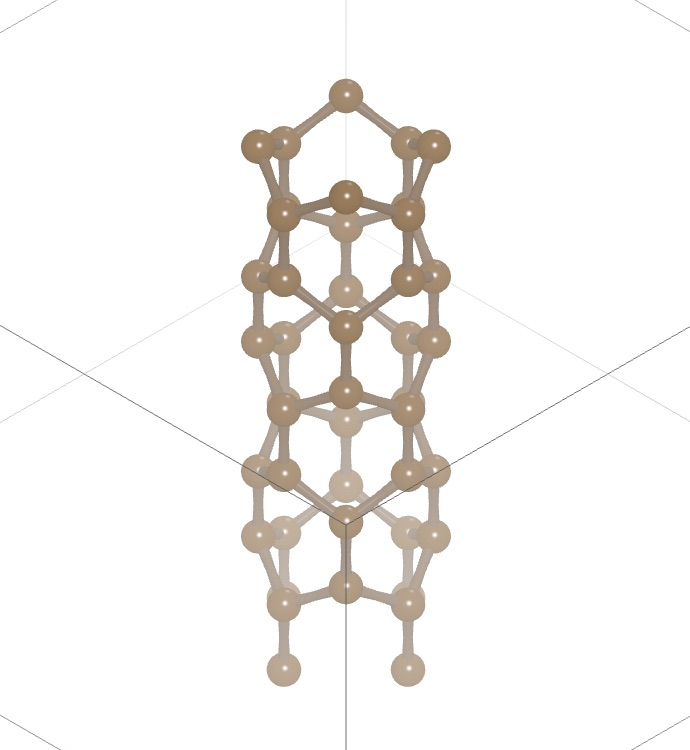
\includegraphics[width=.47\linewidth]{publication-assets/revision-nanotube-perspective.png}\hfill
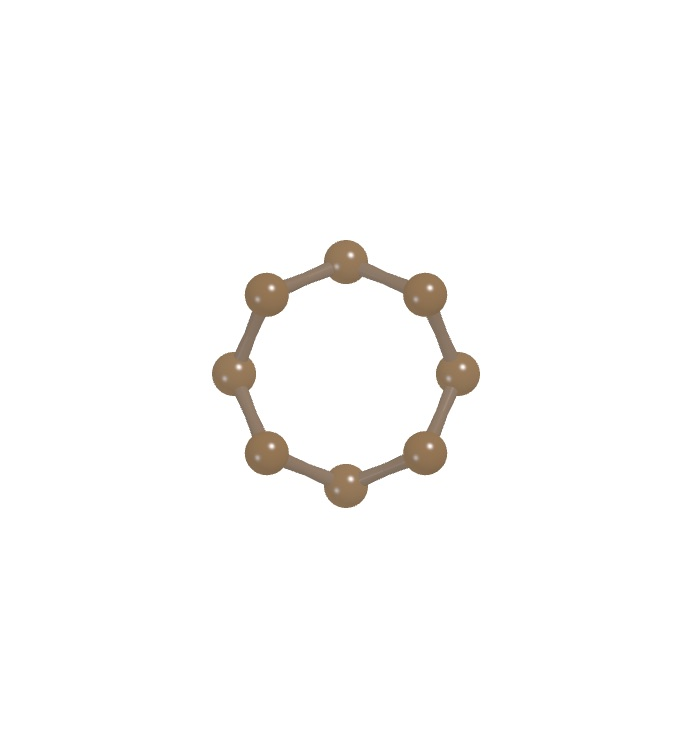
\includegraphics[width=.47\linewidth]{publication-assets/revision-nanotube-axis-c.png}
\caption{同一32位点碳纳米管的三维视图。左：从侧面检查曲面的碳网络和轴向连接；右：沿管口方向观察中央空心区域。显示中包含周期边界映像，独立位点数保持32。}
\label{fig:nanotube-live}
\end{figure}

\FloatBarrier
\subsection{从铜晶体截取纳米线}

铜例子使用随书\file{nano-Cu-fcc-input.json}，与\file{Cu-fcc.cif}来自相同的四位点面心立方晶胞，晶格常数为 $3.61\,\text{\AA}$。纳米线保留一个晶格方向的平移周期，横截面则按给定半径截取。截取球或圆柱时，原子不是连续分布的介质；实际最外原子的跨度不一定等于两倍输入半径。

周期方向指数$[u\,v\,w]$通过实空间晶格给出线轴方向：
\begin{equation}
  \mathbf t=u\mathbf a+v\mathbf b+w\mathbf c.
  \label{eq:nanowire-lattice-direction}
\end{equation}
$u,v,w$为无量纲整数，$\mathbf t$与晶格矢量使用相同的长度单位。构建时取与$\mathbf t$平行的轴，再以给定半径保留横截面内的原子；轴向周期长度以输出晶胞为准。

\begin{table}[htbp]
\centering
\caption{晶格方向指标与晶面指标的区别。}
\begin{tabularx}{\linewidth}{lX}
\toprule
输入 & 对应的几何关系与用途\\
\midrule
$[u\,v\,w]$方向 & 由实空间的$\mathbf a,\mathbf b,\mathbf c$组合得到，用于纳米线轴向等方向选择。\\
$(hkl)$晶面 & 由倒格矢组合得到法向，见式\eqref{eq:surface-miller-normal}，用于表面切割。\\
\bottomrule
\end{tabularx}
\end{table}

在立方晶胞中，同一组三个整数给出的方向与同指数晶面的法向平行；在一般斜晶胞中并非如此。填写前先看窗口要求的是方向还是晶面，再从轴向和侧向检查预览。

\begin{steps}
  \item 导入铜输入并激活，在\ui{纳米结构}中打开\ui{截取纳米线}。
  \item 在\ui{周期方向指数（u v w）}的三个框中分别填0、0、1；半径设为 $3\,\text{\AA}$，轴向重复单元数设为2，真空层厚度设为 $4\,\text{\AA}$，最大原子数设为2000。
  \item 预览时沿线轴观察截面，确认原子位于选定圆柱内。再从侧面看轴向接续，核对共有24个Cu位点。
  \item 应用并保存为\file{Cu-wire-001-r3-l2}。改变半径或方向时，从原始铜晶体重新开始，避免把有限横截面再次当成块体截取。
\end{steps}

结果沿 $z$ 轴周期，周期标记为\literalinput{false false true}，轴向胞长为 $7.22\,\text{\AA}$。两个横向原子跨度均为 $5.415\,\text{\AA}$，加上两侧各 $4\,\text{\AA}$ 的空白后，两个横向盒长均为 $13.415\,\text{\AA}$。最短周期近邻距离约 $2.552655\,\text{\AA}$，与输入面心立方铜的最近邻距离相同。

最大原子数同时约束构建时需要的母超胞规模。本例采用2000；若上限过小，按提示检查母超胞的规模后再调整。

\begin{figure}[!htb]
\centering
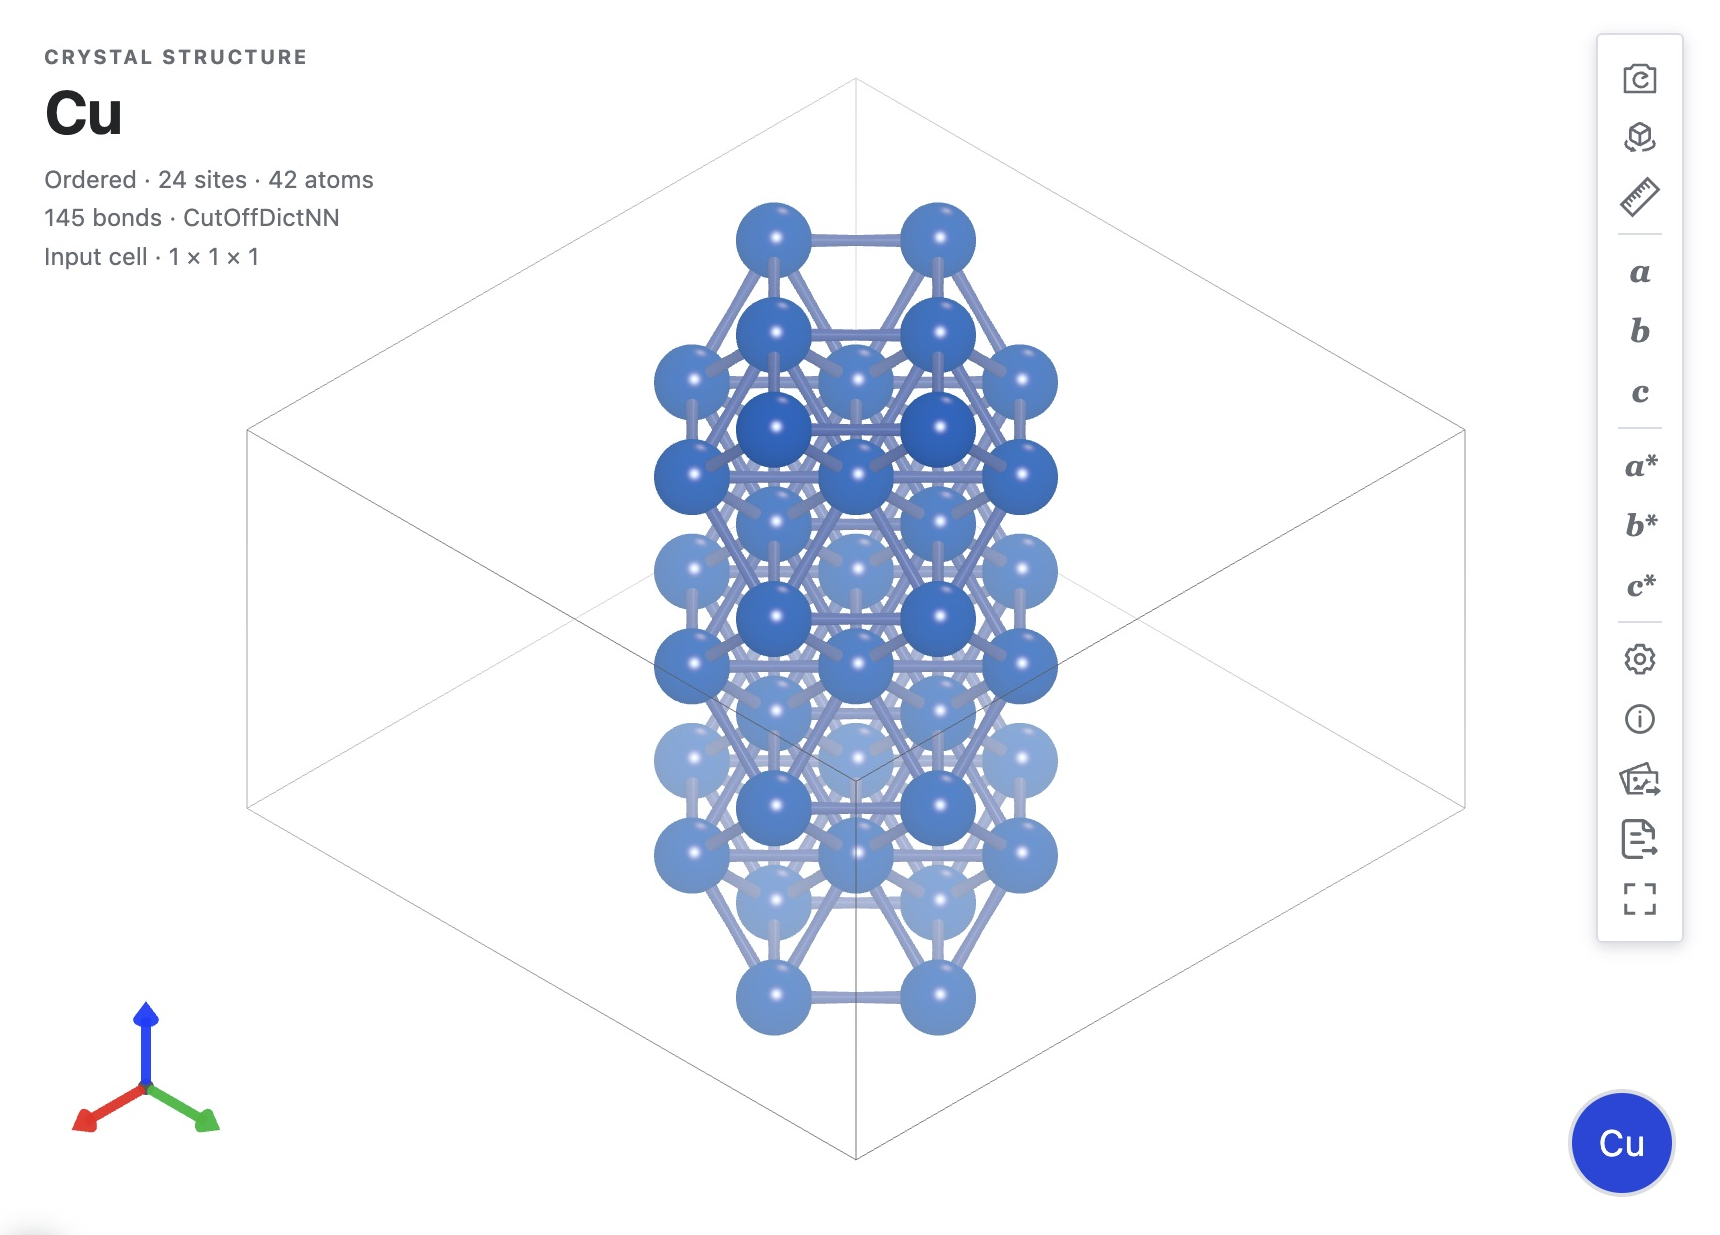
\includegraphics[width=\linewidth]{publication-assets/revision-nanowire-perspective.png}
\caption{随书24位点铜纳米线的实际显示。查看器补出周期边界原子以展示轴向连接，横向的空白属于真空区域。}
\label{fig:nanowire-live}
\end{figure}

\FloatBarrier
\subsection{检查纳米线的截面与轴向}

打开随书\file{Cu-wire-001-r3-l2.json}，即可检查已经截取的24位点铜纳米线。它与纳米管都沿$c$方向周期。纳米管由单层卷成空心圆周；铜纳米线保留圆柱范围内的晶体原子，横截面内部也有原子。

\begin{steps}
  \item 导入JSON并打开三维文档，保持\ui{Input cell}。核对元素为Cu、独立位点为24。
  \item 单击视图工具栏的\ui{c}沿线轴观察截面。原子排列在离散的晶格位置上，轮廓可以呈阶梯状，不必形成光滑圆边。
  \item 单击\ui{a}或\ui{b}看侧面，打开\ui{Unit cell}。用轴向$7.22\,\text{\AA}$与横向$13.415\,\text{\AA}$的盒长解释取景：沿轴向是重复周期，横向大盒用于容纳有限截面与真空。
  \item 清除无关选择，稍微旋转为同时看见截面和侧面的斜视图。保留晶胞边框与方位标记，检查没有原子被视图边缘裁掉。
  \item 按需要将\ui{Repeat cell}的\ui{c}设为2查看接续，随后恢复一个周期。保存项目与结构；导出图片时在图注记录$[001]$方向、输入截取半径$3\,\text{\AA}$和24个位点。
\end{steps}

输入半径决定保留哪些晶格位置，图中最外原子的跨度则由实际保留的离散位置决定。本例横向跨度$5.415\,\text{\AA}$小于直径$6\,\text{\AA}$，与截取规则一致。后续结构优化及电子性质分析可使用相应计算工作流。

\subsection{截取一个有限铜团簇}
\index{Liangzidian@量子点}

\ui{量子点 / 纳米空洞}的\ui{量子点}模式保留球内原子，建立三个方向均不周期的有限结构。本例用13位点铜团簇观察有限边界与周期块体的区别，保存后可继续安排相应的电子结构计算。

\begin{steps}
  \item 重新激活四位点铜输入，从\ui{纳米结构}打开\ui{量子点 / 纳米空洞}。
  \item 处理方式选择\ui{量子点}，半径填 $3\,\text{\AA}$，真空层厚度填 $4\,\text{\AA}$，最大原子数设为2000。
  \item 预览后旋转观察，确认没有一条方向继续连接成无限原子链。检查共有13个Cu位点。
  \item 应用并命名为\file{Cu-dot-r3}，保存项目和结构。
\end{steps}

本例的三个胞长均约为 $11.61\,\text{\AA}$，原子在各方向的跨度均为 $3.61\,\text{\AA}$，三向周期标记均为false。最短原子间距约 $2.552655\,\text{\AA}$。按 $2.8\,\text{\AA}$ 的近邻界限检查，中心原子有12个近邻，其余12个表面原子各有5个近邻。这一初始团簇从面心立方排列直接裁取，稳定构型需进一步优化。

\subsection{在周期铜中挖出球形空洞}
\index{Namikongdong@纳米空洞}

空洞模式保留球外宿主和原周期盒；它与保留球内原子的量子点模式正好相反。先建立足够大的宿主，可以避免只从很小晶胞中删去大部分甚至全部原子。

\begin{steps}
  \item 导入随书\file{Cu-void-host-2x2x2.json}，或从四位点铜输入通过\ui{构建超胞}建立 $2\times2\times2$ 宿主。应有32个Cu位点，三个胞长均为 $7.22\,\text{\AA}$。
  \item 激活这份宿主，打开\ui{量子点 / 纳米空洞}，处理方式选择\ui{纳米空洞}，半径设为 $2.7\,\text{\AA}$。空洞模式不需要为有限团簇增加外部真空。
  \item 预览并显示晶胞边框。空洞中心固定在宿主的分数坐标 \((0.5,0.5,0.5)\)，应检查晶胞中央的原子被移除，而外围周期宿主仍保留。
  \item 核对本例移除13个原子，剩余19个Cu位点；晶格仍为 $7.22\,\text{\AA}$ 的立方胞，三个方向继续周期。
  \item 应用后另存为\file{Cu-void-r2p7}，保留完整32位点宿主，便于以后改变半径或比较缺陷。
\end{steps}

剩余原子距空洞中心的最短周期距离为 $3.61\,\text{\AA}$。这个值大于输入半径 $2.7\,\text{\AA}$，反映了晶格上可保留的位置是离散的，不表示半径字段失效。剩余宿主的最短原子间距仍约 $2.552655\,\text{\AA}$。保存时同时记录“输入删除球半径”和“剩余最近原子距中心”，会比只给一张透视图更清楚。

\subsection{检查周期并保存配套文件}

每个例子的原生JSON保留当前晶格、坐标、周期标记及相应构建信息；CIF用于交换晶胞和原子几何。导入本组CIF时，三个方向均按周期处理。继续低维建模并保留本节的周期方向时，应使用JSON。

\begin{table}[htbp]
\centering\small
\caption{随书纳米结构的位点数与原生周期。}
\begin{tabularx}{\linewidth}{lX}
\toprule
结果 & 实际模型与主要检查值\\
\midrule
石墨烯纳米带 & 24C；仅$y$周期；轴向 $8.521690\,\text{\AA}$。\\
$(4,0)$纳米管 & 32C；仅$z$周期；半径 $1.566085\,\text{\AA}$。\\
铜纳米线 & 24Cu；仅$z$周期；轴向 $7.22\,\text{\AA}$。\\
铜团簇 & 13Cu；三个方向非周期；盒长各 $11.61\,\text{\AA}$。\\
带空洞的铜 & 19Cu；三个方向周期；32位点宿主中移除13个。\\
\bottomrule
\end{tabularx}
\end{table}

\begin{steps}
  \item 先保存项目，确认输入结构和派生结果具有不同名称。
  \item 如需单独结构文件，在查看器的\ui{Export file}\,$\rightarrow$\,\ui{Structure file}中选JSON，保留模型信息；几何交换可另存CIF。这里不要选择用于显示场景的\ui{Scene JSON}。
  \item 重新打开保存的结构，检查位点数、晶胞和周期方向；再检查边缘、卷合处或球形裁切边界的近邻。
  \item 需要重新生成这组结构时，以\file{-nojvm}启动MATLAB\regmark{}，配置好工具箱路径后，从随书示例目录运行\file{nano_examples.m}。\file{verify_nano_examples.m}用于检查已有结构。
\end{steps}

本节提供未钝化的初始模型，可根据材料与边界需要继续钝化、弛豫和电子结构计算。将模型接入工作流时，保存构建参数与计算参数，并确认工作流引用所需的结构。
